\section{Introduction}
In previous chapters, we used variable, arrays and structures to store the data; but such data do not store permanently and lost after the termination of the program. Data can be stored to file using keyword `fwrite'; and can be read from the file using keyword `fscanf', as shown in this chapter. 


\section{Write data to file}
For writing or reading data from a file, we need to create one `FILE pointer' as shown in Line 10 of Listing \ref{c:writeDataEx}. Next, we need to open the file, which is done at Line 13; this line prints the message at Line 14, if the file can not be open. Note that, the file `data.txt' file is saved inside the `data' folder, therefore we need to create the `data' folder first, as compiler can not create the folder. If file is open successfully, the compiler will reach to `else' block at Line 16; where it will read the data from the terminal (Line 19), and then save it to file using `fprintf' command at Line 22. The `while loop' is used at Line 21, which reads the data from terminal until `end of file command' is given i.e. ``ctrl-Z'' or ``crtl-C'', as shown in Fig. \ref{fig:writeDataEx}. The data saved by the listing is shown in Fig. \ref{fig:writeDataEx2}. 


\lstinputlisting[
language = C,
caption    = {Write data to file},
label      = {c:writeDataEx}
]{writeDataEx.c}

\begin{figure}[!h]
	\centering
	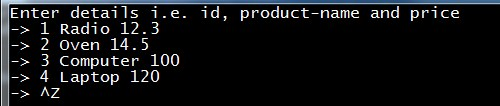
\includegraphics{writeDataEx}
	\caption{Reading data from terminal}
	\label{fig:writeDataEx}
\end{figure}

\begin{figure}[!h]
	\centering
	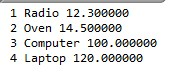
\includegraphics{writeDataEx2}
	\caption{Data in `data.txt' file}
	\label{fig:writeDataEx2}
\end{figure}

\section{Read data from file}
Reading operation is similar to writing operation. The `fscanf' command is used to read the data from the file, as shown in Line 16 and 20 of Listing \ref{c:readDataEx}. 

\lstinputlisting[
language = C,
caption    = {Read data from file},
label      = {c:readDataEx}
]{readDataEx.c}

\section{Conclusion}
In this chapter, we learn to read and write data to file. We can permanently store the data to file using `fwrite command'; and then this data can be processed and analyzed by some other software like Python and R etc. 